\documentclass{article}
\usepackage{graphicx}

\begin{document}

\begin{titlepage}
\title{ECS189G Homework 3 Report Problem B}
\author{Goh Chang Kang, Charles 916751838, \\
Yang Minxing 916751773, Chen Jieyi Chloe 999823783}

\date{November 15, 2018}
\maketitle
\end{titlepage}


\section{Problem B}
Before we test the effect of using covariates and not using covariates on the MAPE with varying levels of maximum items, we had to find out what was the best weight to use for the covariates:
\begin{verbatim}
mLists <- c()
withoutCov <- c()
withCov <- c()
differences <- c()


lapply(c(0.5, 1, 5, 10), function(wtcovs_input) {
  m = 5
  k = 10
  output = form_df(ivl_formed, m)
  train_formed_without_covariates = output[[1]]
  test_formed_without_covariates = output[[2]]
  
  train_formed_with_covariates = output[[3]]
  test_formed_with_covariates = output[[4]]
  
  error_output = result_comparison(m, k, 
  test_formed_without_covariates, train_formed_without_covariates, 
  test_formed_with_covariates, train_formed_with_covariates, wtcovs_input)
  mLists <<- c(mLists, m)
  withoutCov <<- c(withoutCov, error_output[[1]])
  withCov <<- c(withCov, error_output[[2]])
  differences <<- c(differences, error_output[[1]] - error_output[[2]])
})

\end{verbatim}

Our results are shown below. We found that an estimated optimum for the weight placed on covariates should be 1, as it returns results with the greatest MAPE value differences.

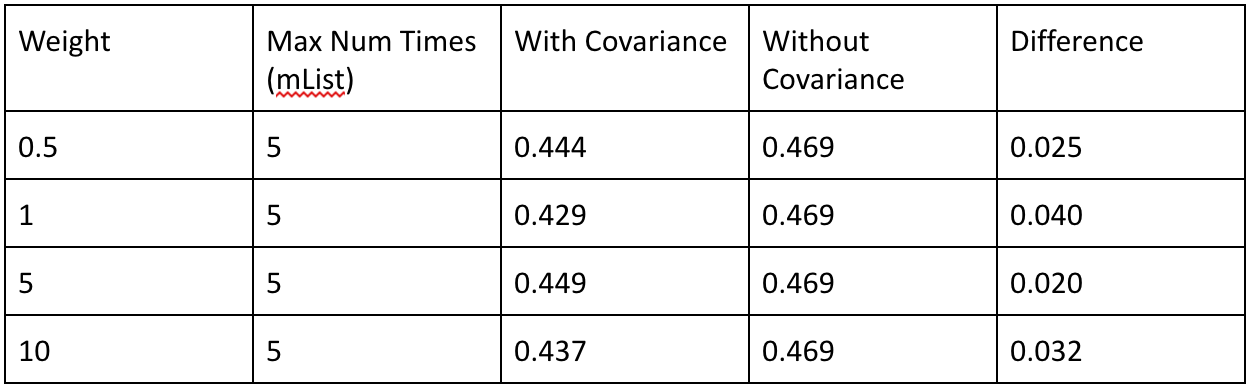
\includegraphics[scale=0.5]{FindingCovariateWeights.png}

Now we can begin testing predictions using covariates and not using covariates with varying levels of maximum items. 

\begin{verbatim}
library(rectools)
#setwd("/Users/yangminxing/libimseti")

# Problem B
getInstEval()
ivl_formed = formUserData(ivl[, c(1, 2, 3)])

# Gets users where number of ratings are less than parameter num_rating
form_df = function(ivl_formed, num_rating){
  # get the number of ratings for each userID
  length_output = sapply(ivl_formed, function(dbElement) length(dbElement$ratings))
  # filter the ivl dataframe on a vector with userID that has rating items 
  # less than num_rating
  test_set = subset(ivl, s %in% names(which(length_output <= num_rating)))
  train_set = subset(ivl, !(s %in% names(which(length_output <= num_rating))))
  train_formed_without_covariates = formUserData(train_set[, 1:3])
  test_formed_without_covariates = formUserData(test_set[, 1:3])
  user_coariates = train_set[, 4:19]
  train_formed_with_covariates = formUserData(train_set[, 1:3], usrCovs = user_coariates)
  test_formed_with_covariates = formUserData(test_set[, 1:3], usrCovs = user_coariates)
  return (list(train_formed_without_covariates, test_formed_without_covariates, 
  train_formed_with_covariates, test_formed_with_covariates))
}

# Predict auxillary function. wtcovs is null when no covariates
predict_df = function(test_formed, trainset_input, k, wtcovs){
  #Initialize relevant variables
  usr_id <- vector()
  actual <- vector()
  predict <- vector()
  difference <- vector()
  
  # loop over each row in the test_formed data
  lapply(test_formed, function(usr) {
    # get the total number of ratings for each user ID
    itmNumList <- 1:length(usr$ratings)
    # iterate through each item in the item list
    lapply(itmNumList, function(num) {
      #remove the record from the user to predict
      holdRating = usr$ratings[[num]] 
      # set the temporary variable to store the existing items and ratings
      tmpUsr <- usr
      tmpUsr$itms <- usr$itms[-num] 
      tmpUsr$ratings <- usr$ratings[-num] 
      result <- predict(trainset_input,tmpUsr,usr$itms[num],k, wtcovs)
      diff = result - holdRating
      usr_id <<- c(usr_id, usr$userID)
      actual <<- c(actual, holdRating)
      predict <<- c(predict, result)
      difference <<- c(difference, diff)
    })
  })
  
  Result <- data.frame(
    usr_id,
    actual,
    predict,
    difference
  )
}

## calculate the MAPE error
MAPE = function(df_list) {
  error_percentage = sum(abs(df_list['difference'])/abs(df_list['actual']))/nrow(df_list) 
  return (round(error_percentage, 3))
}

# Process and returns results with and without covariates
result_comparison = function(num_rating, k, test_formed_without_covariates, 
train_formed_without_covariates, test_formed_with_covariates, 
train_formed_with_covariates, wtcovs_input){
  Result_without_covariates = predict_df(test_formed_without_covariates, 
  train_formed_without_covariates, k, wtcovs = NULL)
  Result_with_covariates = predict_df(test_formed_with_covariates, 
  train_formed_with_covariates, k, wtcovs = wtcovs_input)
  error_without_covariates = MAPE(Result_without_covariates)
  error_with_covariates = MAPE(Result_with_covariates)
  return(list(error_without_covariates, error_with_covariates))
}

# Set up data structure to capture results
mLists <- c()
withoutCov <- c()
withCov <- c()
differences <- c()
wtcovs_input = 1

# For maximum ratings from 5 to 10, we predict with and 
#without covariates and then compare MAPE values
lapply(5:10, function(m) {
  k = 10
  output = form_df(ivl_formed, m)
  train_formed_without_covariates = output[[1]]
  test_formed_without_covariates = output[[2]]
  
  train_formed_with_covariates = output[[3]]
  test_formed_with_covariates = output[[4]]
  
  error_output = result_comparison(m, k, test_formed_without_covariates, 
  train_formed_without_covariates, test_formed_with_covariates, 
  train_formed_with_covariates, wtcovs_input)
  mLists <<- c(mLists, m)
  withoutCov <<- c(withoutCov, error_output[[1]])
  withCov <<- c(withCov, error_output[[2]])
  differences <<- c(differences, error_output[[1]] - error_output[[2]])
})

draw <- data.frame(
  mLists,
  differences,
  withCov,
  withoutCov
)

# Now we plot the graph
library(ggplot2)
plot_graph = function(dataframe, data_col, colname){
  ggplot(dataframe, aes(x = factor(mLists, levels = dataframe$mLists),
                        y = data_col)) +
    geom_bar(stat = 'identity', fill = 'steelblue') +
    geom_text(aes(label = data_col), vjust = -0.5, color = "black") +
    xlab('m_value') +
    ylab(colname)
}

plot_graph(draw, draw$difference, 'difference')
\end{verbatim}

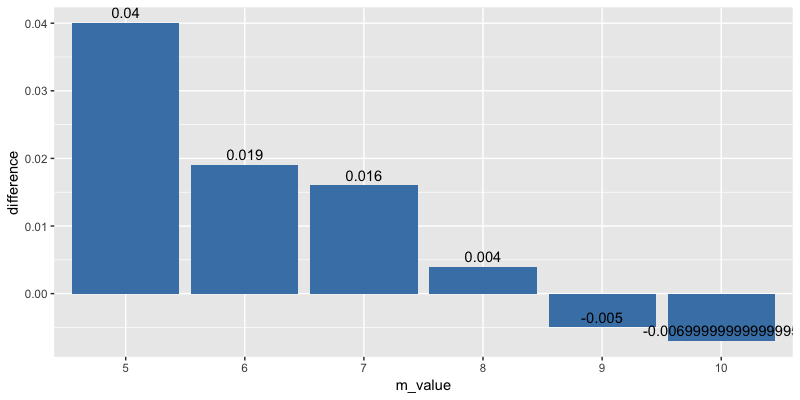
\includegraphics[scale=0.5]{WithAndWithoutCovariatesMAPEComparison.png}

The chart above shows how much the MAPE values for the results without the covariates differs from the results with the covariates (i.e. without results - with results). We can observe that the MAPE values for the without covariates results is higher than the MAPE values for the with covariates results when m = 5, indicating that covariates play a positive role in the prediction when maximum ratings is small. However, this effect appears to lessen as the maximum ratings increases, resulting in it becoming noise when maximum ratings is 10 and above. 

\end{document}